\documentclass[pdf]{beamer}
\usepackage{lmodern}
\mode<presentation>{\usetheme{PaloAlto}}
\title{Speckle Interferometry}
\author{Matt Rauen and David Fan}
\date{\today}
\begin{document}
\begin{frame}
\titlepage
\end{frame}

\section{Abstract}
\begin{frame}{Abstract}

\end{frame}

\section{Research Questions}
\begin{frame}{Research Questions}
\begin{center}
Primary Question:

How does the piezo deform when a voltage is applied to it?
\end{center}
More concretely, we want to construct a topological map of the shift at each point, where each point is characterized by the phase difference (relative to the wavelength of light we used) between its original position and its position after the applied voltage.
\begin{figure}[htbp]
\centering
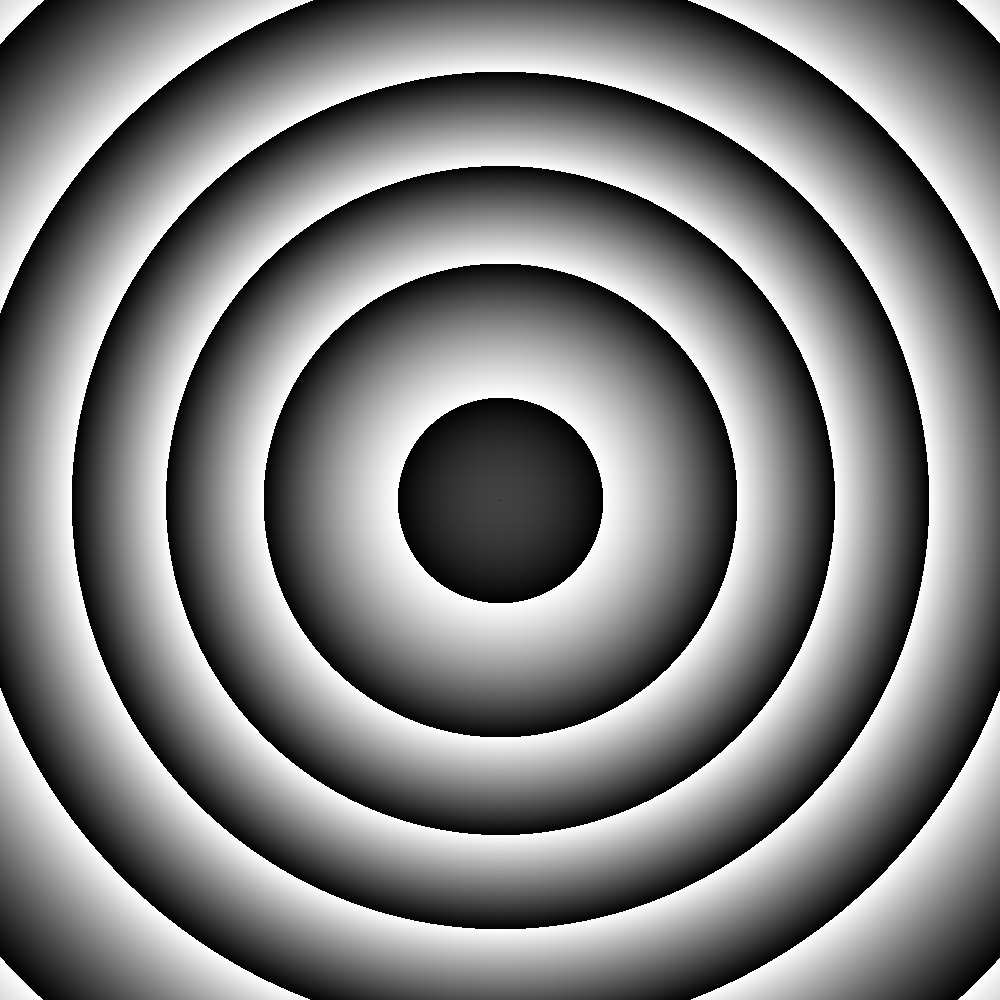
\includegraphics[width=0.3\textwidth]{gaussian_bump.png}
\end{figure}
\end{frame}

\section{Background}
\begin{frame}{Speckle Patterns}

\end{frame}

\begin{frame}{Modeling Each Speckle}
We can model the intensity of each pixel via the equation$$A\cos x + b_0,$$where $A$ and $b_0$ are fixed constants, and $x$ is proportional to the distance between the aperture and the piezo at that pixel.\\
\vspace{0.5cm}
Therefore, if we translate the reference object, while holding the object of interest stationary, we would expect that the intensities of any given pixel trace out a cosine curve with some offset.
\end{frame}

\section{Setup}
\begin{frame}{Setup}

\end{frame}

\section{Analysis}
\begin{frame}{Calculating Absolute Phases}

\end{frame}

\begin{frame}{Calculating Absolute Phases}

\end{frame}

\begin{frame}{Calculating Relative Phases}

\end{frame}

\section{Results}
\begin{frame}{Results}

\end{frame}

\section{Conclusions}
\begin{frame}{Conclusions}

\end{frame}

\section{Future Research}
\begin{frame}{Future Research}
Some additional directions in which this could be taken include:
\begin{itemize}
\item{Visualizing the behavior of membrane oscillations, by computing the relative phase differences of the surface at several moments during the oscillation.}
\item{Analyzing the stress that can be handled by a material. This could be done by applying a force, looking at the phase shifts, and looking for discontinuities that would imply cracking.}
\item{The approach itself could be improved by using more sophisticated cosine fitting algorithms to reduce the error from fitting a cosine to three points.}
\end{itemize}
\end{frame}

\section{References}
\begin{frame}{References}

\end{frame}
\end{document}